%========================================================================================
%  Seção 16.2 do D2L -- Sentiment Analysis: Using Recurrent Neural Networks
%  https://d2l.ai/chapter_natural-language-processing-applications/sentiment-analysis-rnn.html
%========================================================================================

%------------------------------------------------
\section{Análise de sentimento com RNN}
%------------------------------------------------

\begin{frame}{Aplicação: análise de sentimento com RNN}
    \begin{columns}[c]
        \begin{column}{0.52\textwidth}
            \footnotesize
            \begin{itemize}
                \item Tarefa: uma frase de \textbf{tamanho variável} entra, uma \textbf{classe fixa} sai: positivo ou negativo.
                \item Dados (Seção 16.1): críticas de filmes do \textbf{IMDb}, 25 mil para treino e 25 mil para teste, metade positivas e metade negativas.
                \item Cada crítica é cortada ou completada com \texttt{<pad>} até \textbf{500 tokens}; lotes de 64 críticas.
                \item A ideia da Seção 16.2: reaproveitar os \textbf{vetores pré-treinados} do GloVe numa \textbf{RNN}.
            \end{itemize}
        \end{column}
        \begin{column}{0.46\textwidth}
            \centering
            \begin{tikzpicture}[font=\scriptsize,
                critica/.style={draw=dexpiBlue, fill=dexpiBlueLight, rounded corners=2pt, text width=3.6cm, align=left, inner sep=3pt},
                rot/.style={rounded corners=2pt, font=\scriptsize\bfseries, inner sep=3pt}]
                \node[critica] (c1) at (0,0.8) {``this movie is so great, i loved every minute''};
                \node[critica] (c2) at (0,-0.6) {``this movie is so bad, a waste of time''};
                \node[rot, draw=dexpiGreenDark, fill=dexpiGreenLight, text=dexpiGreenDark] (r1) at (3.0,0.8) {positivo};
                \node[rot, draw=dexpiRedDark, fill=dexpiRedLight, text=dexpiRedDark] (r2) at (3.0,-0.6) {negativo};
                \draw[-{Stealth}, thick, dexpiBlue] (c1) -- (r1);
                \draw[-{Stealth}, thick, dexpiBlue] (c2) -- (r2);
            \end{tikzpicture}
        \end{column}
    \end{columns}
    \vspace{0.3cm}
    \centering
    \begin{tikzpicture}[font=\scriptsize,
        etapa/.style={rounded corners=3pt, minimum width=3.4cm, minimum height=1.0cm, align=center, thick},
        s/.style={-{Stealth}, very thick, gray}]
        \node[etapa, draw=dexpiGreenDark, fill=dexpiGreenLight] (a) at (0,0) {\textbf{Pré-treino}\\GloVe (Seção 15.5)};
        \node[etapa, draw=dexpiBlue, fill=dexpiBlueLight] (b) at (4.4,0) {\textbf{Arquitetura}\\RNN bidirecional (BiRNN)};
        \node[etapa, draw=dexpiRedDark, fill=dexpiRedLight] (c) at (8.8,0) {\textbf{Aplicação}\\análise de sentimento};
        \draw[s] (a) -- (b);
        \draw[s] (b) -- (c);
    \end{tikzpicture}

    \note{
        Até aqui falamos de como aprender bons vetores de palavras. Agora vamos usar esses vetores numa aplicação de verdade: a análise de sentimento, da Seção 16.2 do livro.
        A tarefa é simples de enunciar: entra uma frase de tamanho variável, sai uma classe fixa, positivo ou negativo. ``This movie is so great'' é positivo; ``this movie is so bad'' é negativo.
        Os dados, preparados na Seção 16.1, são críticas de filmes do site IMDb: 25 mil para treino e 25 mil para teste, metade positivas e metade negativas. Como as críticas têm tamanhos diferentes, cada uma é cortada ou completada com um token de preenchimento até ter exatamente 500 tokens, e o treino usa lotes de 64 críticas.
        A figura de baixo, que segue a Figura 16.2.1 do livro, resume a ideia da seção: pegamos os vetores pré-treinados do GloVe, colocamos numa arquitetura de rede recorrente bidirecional e aplicamos na análise de sentimento.
    }
\end{frame}

\begin{frame}{A arquitetura BiRNN: três camadas}
    \centering
    \begin{tikzpicture}[font=\scriptsize,
        cam/.style={rounded corners=2pt, align=center, minimum height=1.1cm, inner sep=3pt, thick},
        s/.style={-{Stealth}, thick, dexpiBlue},
        dim/.style={font=\tiny, text=dexpiRedDark}]
        \node[draw=gray, rounded corners=2pt, align=center, minimum height=1.1cm, inner sep=3pt] (x) at (0,0) {índices das\\palavras};
        \node[cam, draw=dexpiGreenDark, fill=dexpiGreenLight] (e) at (2.75,0) {\textbf{Embedding}\\{\tiny\texttt{self.embedding}}\\{\tiny (GloVe, $d = 100$)}};
        \node[cam, draw=dexpiBlue, fill=dexpiBlueLight] (l) at (5.85,0) {\textbf{LSTM bidirecional}\\{\tiny\texttt{self.encoder}}\\{\tiny 2 camadas, 100 unidades}};
        \node[cam, draw=dexpiBlue, fill=white] (c) at (8.75,0) {\textbf{concatena}\\{\tiny 1.º e último}\\{\tiny passos}};
        \node[cam, draw=dexpiRedDark, fill=dexpiRedLight] (d) at (11.2,0) {\textbf{Linear}\\{\tiny\texttt{self.decoder}}\\{\tiny $400 \to 2$}};
        \draw[s] (x) -- node[below=0.62cm, dim] {(B, T)} (e);
        \draw[s] (e) -- node[below=0.62cm, dim] {(T, B, 100)} (l);
        \draw[s] (l) -- node[below=0.62cm, dim] {(T, B, 200)} (c);
        \draw[s] (c) -- node[below=0.62cm, dim] {(B, 400)} (d);
        \draw[s] (d.east) -- ++(0.6,0) node[right, align=left, font=\tiny] {pos.\\neg.};
    \end{tikzpicture}

    \vspace{0.3cm}
    \raggedright
    \footnotesize
    \begin{itemize}
        \item \textbf{Embedding}: troca o índice de cada palavra pelo seu vetor denso (aqui, o vetor do GloVe).
        \item \textbf{Codificador}: uma \textbf{LSTM bidirecional} lê a frase nos dois sentidos e gera um estado oculto por palavra.
        \item \textbf{Decodificador}: uma camada \texttt{nn.Linear} transforma a representação da frase em \textbf{2 \textit{logits}} (positivo e negativo).
    \end{itemize}
    {\scriptsize B = tamanho do lote (64), T = número de passos (500). A LSTM do PyTorch quer o tempo na 1.ª dimensão, por isso a entrada é transposta.}

    \note{
        O modelo do livro, chamado BiRNN, tem três camadas, e a figura mostra o caminho de um lote de críticas por elas, com o formato dos tensores em vermelho.
        A entrada são os índices das palavras: um lote de B críticas, cada uma com T tokens. B é 64 e T é 500.
        A primeira camada é o embedding: troca cada índice pelo vetor da palavra. Aqui, esses vetores vão ser os do GloVe, de dimensão 100. Um detalhe de implementação: a LSTM do PyTorch espera o tempo na primeira dimensão, então a entrada é transposta, e o formato vira T por B por 100.
        A segunda camada é o codificador: uma LSTM bidirecional, com 2 camadas empilhadas e 100 unidades ocultas. Ela gera um estado oculto para cada palavra. Como são duas direções, cada estado tem 200 números: 100 da leitura para a frente e 100 da leitura para trás.
        Depois vem o passo mais interessante, que vamos ver com calma: juntamos os estados do primeiro e do último passo de tempo, o que dá um vetor de 400 números por crítica.
        Por fim, o decodificador: uma camada linear que leva esses 400 números a 2 saídas, os logits de positivo e de negativo.
    }
\end{frame}

\begin{frame}{Por que LSTM? Por que bidirecional?}
    \begin{columns}[t]
        \begin{column}{0.48\textwidth}
            \begin{block}{Por que LSTM?}
                \footnotesize
                \begin{itemize}
                    \item Uma RNN simples sofre com o \textbf{gradiente que desvanece}: ela ``esquece'' o começo de frases longas.
                    \item A LSTM tem \textbf{portões} que decidem o que guardar e o que esquecer, e lembra de contextos distantes.
                \end{itemize}
                \centering
                \begin{tikzpicture}[font=\scriptsize]
                    \node[anchor=base] (f) at (0,0) {o \textbf{filme},};
                    \node[anchor=base, text=gray] (m) at (2.1,0) {apesar do começo lento,};
                    \node[anchor=base] (o) at (4.2,0) {é \textbf{ótimo}};
                    \draw[-{Stealth}, thick, dexpiGreenDark] (o.north) to[bend right=25] node[above, font=\tiny, text=dexpiGreenDark] {a LSTM liga os dois} (f.north);
                \end{tikzpicture}
            \end{block}
        \end{column}
        \begin{column}{0.50\textwidth}
            \begin{block}{Por que bidirecional?}
                \footnotesize
                \begin{itemize}
                    \item Duas LSTMs em paralelo: uma lê para a \textbf{frente}, outra para \textbf{trás}.
                    \item O sentido de uma palavra depende da \textbf{direita} tanto quanto da \textbf{esquerda}.
                \end{itemize}
                \centering
                \begin{tikzpicture}[font=\tiny,
                    w/.style={minimum width=0.85cm, inner sep=1pt},
                    fw/.style={draw=dexpiBlue, fill=dexpiBlueLight, minimum width=0.85cm, minimum height=0.38cm, inner sep=0pt},
                    bw/.style={draw=dexpiRedDark, fill=dexpiRedLight, minimum width=0.85cm, minimum height=0.38cm, inner sep=0pt}]
                    \foreach \p [count=\k from 1] in {o, filme, é, bom} {
                        \node[w, font=\scriptsize] (w\k) at ({1.05*\k},0) {\p};
                        \node[fw] (f\k) at ({1.05*\k},0.65) {$\overrightarrow{\mathbf{h}}_{\k}$};
                        \node[bw] (b\k) at ({1.05*\k},1.25) {$\overleftarrow{\mathbf{h}}_{\k}$};
                    }
                    \foreach \i/\j in {1/2,2/3,3/4} {
                        \draw[-{Stealth}, dexpiBlue] (f\i) -- (f\j);
                        \draw[-{Stealth}, dexpiRedDark] (b\j) -- (b\i);
                    }
                    \node[anchor=west, text=dexpiBlue] at (4.55,0.65) {frente};
                    \node[anchor=west, text=dexpiRedDark] at (4.55,1.25) {trás};
                \end{tikzpicture}
            \end{block}
        \end{column}
    \end{columns}
    \vspace{0.2cm}
    \footnotesize
    Saída em cada palavra: $\mathbf{h}_t = [\,\overrightarrow{\mathbf{h}}_t\,;\,\overleftarrow{\mathbf{h}}_t\,]$, com $100 + 100 = 200$ números.

    \note{
        Por que essa escolha de camada? Duas perguntas: por que LSTM, e por que bidirecional?
        Por que LSTM: uma rede recorrente simples sofre com o gradiente que desvanece. Na prática, isso quer dizer que ela esquece o começo de frases longas. A LSTM, Long Short-Term Memory, tem portões que decidem o que guardar na memória e o que esquecer, e por isso consegue lembrar de contextos distantes. No exemplo: ``o filme, apesar do começo lento, é ótimo''. Para entender que a crítica é positiva, o modelo precisa ligar o ``ótimo'' lá do fim ao ``filme'' do começo, passando por um trecho negativo no meio.
        Por que bidirecional: uma RNN normal lê só da esquerda para a direita. A bidirecional tem duas LSTMs rodando em paralelo: uma lê ``o filme é bom'' para a frente, a outra lê de trás para a frente, ``bom é filme o''. É a mesma ideia que vimos no ELMo: o sentido de uma palavra depende da direita tanto quanto da esquerda.
        Em cada palavra, a saída junta os dois estados, o da frente e o de trás. Com 100 unidades em cada direção, são 200 números por palavra.
    }
\end{frame}

\begin{frame}{O pulo do gato: concatenar o primeiro e o último passo}
    \centering
    \begin{tikzpicture}[font=\tiny,
        fw/.style={draw=dexpiBlue, fill=dexpiBlueLight, minimum width=0.95cm, minimum height=0.4cm, inner sep=0pt},
        bw/.style={draw=dexpiRedDark, fill=dexpiRedLight, minimum width=0.95cm, minimum height=0.4cm, inner sep=0pt},
        fraco/.style={opacity=0.35},
        seg/.style={draw, minimum height=0.42cm, minimum width=1.3cm, inner sep=0pt, font=\tiny}]
        \foreach \p [count=\k from 1] in {this, movie, is, so, great} {
            \node[font=\scriptsize] (w\k) at ({1.25*\k},0) {\p};
            \node[fw] (f\k) at ({1.25*\k},0.6) {$\overrightarrow{\mathbf{h}}_{\k}$};
            \node[bw] (b\k) at ({1.25*\k},1.15) {$\overleftarrow{\mathbf{h}}_{\k}$};
        }
        \foreach \i/\j in {1/2,2/3,3/4,4/5} {
            \draw[-{Stealth}, dexpiBlue] (f\i) -- (f\j);
            \draw[-{Stealth}, dexpiRedDark] (b\j) -- (b\i);
        }
        \node[draw=dexpiGreenDark, very thick, rounded corners, fit=(f1)(b1), inner sep=2pt, label={[font=\scriptsize\bfseries, text=dexpiGreenDark]above:\texttt{outputs[0]}}] {};
        \node[draw=dexpiGreenDark, very thick, rounded corners, fit=(f5)(b5), inner sep=2pt, label={[font=\scriptsize\bfseries, text=dexpiGreenDark]above:\texttt{outputs[-1]}}] {};
        % anotacoes
        \node[anchor=east, align=right, text=dexpiRedDark] at (0.55,1.15) {$\overleftarrow{\mathbf{h}}_1$: leu a frase\\\textbf{toda} (de trás)};
        \node[anchor=east, align=right, text=gray] at (0.55,0.6) {$\overrightarrow{\mathbf{h}}_1$: só viu ``this''};
        \node[anchor=west, align=left, text=dexpiBlue] at (6.95,0.6) {$\overrightarrow{\mathbf{h}}_5$: leu a frase\\\textbf{toda} (da frente)};
        \node[anchor=west, align=left, text=gray] at (6.95,1.15) {$\overleftarrow{\mathbf{h}}_5$: só viu ``great''};
        % vetor concatenado
        \node[seg, draw=dexpiBlue, fill=dexpiBlueLight, fraco] (v1) at (1.95,-0.85) {$\overrightarrow{\mathbf{h}}_1$ (100)};
        \node[seg, draw=dexpiRedDark, fill=dexpiRedLight, right=0pt of v1] (v2) {$\overleftarrow{\mathbf{h}}_1$ (100)};
        \node[seg, draw=dexpiBlue, fill=dexpiBlueLight, right=0pt of v2] (v3) {$\overrightarrow{\mathbf{h}}_5$ (100)};
        \node[seg, draw=dexpiRedDark, fill=dexpiRedLight, fraco, right=0pt of v3] (v4) {$\overleftarrow{\mathbf{h}}_5$ (100)};
        \node[anchor=west, font=\scriptsize] at (v4.east) {\;$= 400 = 4 \times$ \texttt{num\_hiddens}};
        \node[anchor=east, font=\scriptsize\ttfamily] at (v1.west) {encoding =\;};
    \end{tikzpicture}

    \vspace{0.15cm}
    \raggedright
    \footnotesize
    \texttt{encoding = torch.cat((outputs[0], outputs[-1]), dim=1)}
    \begin{itemize}
        \item \texttt{outputs} traz um estado por palavra, \textbf{só da última camada}: cada um tem $2 \times 100 = 200$ números.
        \item As metades que resumem a frase inteira são $\overleftarrow{\mathbf{h}}_1$ e $\overrightarrow{\mathbf{h}}_T$, e cada uma está numa ponta. Por isso pegamos as \textbf{duas pontas}.
        \item O 4 de \texttt{nn.Linear(4 * num\_hiddens, 2)} vem de \textbf{2 passos $\times$ 2 direções}, e não das 2 camadas.
    \end{itemize}

    \note{
        Agora o pulo do gato, a linha mais importante do código: a concatenação do primeiro e do último passo.
        A LSTM bidirecional devolve \texttt{outputs}: um estado oculto para cada palavra da frase. Cada estado tem duas metades, a da leitura para a frente, em azul, e a da leitura para trás, em vermelho.
        Agora pensem no que cada metade já leu. A seta azul anda da esquerda para a direita. Então o h azul da primeira palavra só viu ``this''. Mas o h azul da última palavra leu a frase inteira. A seta vermelha anda ao contrário: o h vermelho da última palavra só viu ``great'', e o h vermelho da primeira palavra leu a frase inteira, de trás para a frente.
        Ou seja, os dois resumos completos da frase estão em pontas opostas: um no fim, outro no começo. Por isso o código pega \texttt{outputs[0]} e \texttt{outputs[-1]} e concatena. O vetor resultante, embaixo, tem as quatro metades. As duas mais apagadas viram pouca coisa, mas vêm junto. As duas fortes resumem a frase nos dois sentidos.
        E isso explica o tamanho: cada passo tem 200 números, dois passos dão 400, que é 4 vezes o número de unidades ocultas. Um cuidado: é comum achar que o 4 vem das 2 camadas vezes 2 direções. Não é. O \texttt{outputs} da LSTM só traz a última camada. O 4 vem de 2 passos de tempo vezes 2 direções.
    }
\end{frame}

\begin{frame}[fragile]{O código da BiRNN}
\vspace{-0.2cm}
\begin{lstlisting}[basicstyle=\ttfamily\fontsize{6.4}{7.6}\selectfont]
class BiRNN(nn.Module):
    def __init__(self, vocab_size, embed_size, num_hiddens, num_layers, **kwargs):
        super(BiRNN, self).__init__(**kwargs)
        self.embedding = nn.Embedding(vocab_size, embed_size)
        self.encoder = nn.LSTM(embed_size, num_hiddens, num_layers=num_layers,
                               bidirectional=True)              # LSTM bidirecional
        self.decoder = nn.Linear(4 * num_hiddens, 2)            # 2 passos x 2 direcoes

    def forward(self, inputs):                                  # inputs: (B, T)
        embeddings = self.embedding(inputs.T)                   # (T, B, 100): tempo primeiro
        self.encoder.flatten_parameters()
        outputs, _ = self.encoder(embeddings)                   # (T, B, 200): so a ultima camada
        encoding = torch.cat((outputs[0], outputs[-1]), dim=1)  # (B, 400): 1o e ultimo passos
        outs = self.decoder(encoding)                           # (B, 2): logits pos./neg.
        return outs

embed_size, num_hiddens, num_layers = 100, 100, 2
net = BiRNN(len(vocab), embed_size, num_hiddens, num_layers)
\end{lstlisting}
\vspace{-0.15cm}
\footnotesize
Os pesos das camadas lineares e da LSTM começam com a inicialização de \textbf{Xavier} (\texttt{init\_weights} no D2L).

\note{
    Este é o código do livro, com comentários dos formatos.
    No construtor, as três camadas: o embedding, a LSTM com \texttt{bidirectional=True}, e a camada linear de 4 vezes \texttt{num\_hiddens} para 2.
    No forward: a entrada chega como B por T e é transposta, porque a LSTM do PyTorch quer o tempo primeiro. O embedding dá T por B por 100. A LSTM devolve \texttt{outputs}, com formato T por B por 200, só da última camada. A chamada \texttt{flatten\_parameters} é só uma otimização de memória para GPU.
    Depois vem a concatenação do primeiro e do último passo, que dá B por 400, e a camada linear, que dá B por 2: os logits de positivo e de negativo.
    Os hiperparâmetros são embedding de dimensão 100, 100 unidades ocultas e 2 camadas. E os pesos começam com a inicialização de Xavier, a mesma que usamos no word2vec.
}
\end{frame}

\begin{frame}[fragile]{Embeddings pré-treinados: o GloVe de 100 dimensões}
    \begin{columns}[c]
        \begin{column}{0.55\textwidth}
\begin{lstlisting}[basicstyle=\ttfamily\fontsize{6.2}{7.2}\selectfont]
glove_embedding = d2l.TokenEmbedding('glove.6b.100d')
embeds = glove_embedding[vocab.idx_to_token]
embeds.shape                 # torch.Size([49346, 100])
net.embedding.weight.data.copy_(embeds)
net.embedding.weight.requires_grad = False  # congela
\end{lstlisting}
            \footnotesize
            \begin{itemize}
                \item Em vez de pesos aleatórios, o embedding começa com vetores que \textbf{já sabem} o significado das palavras.
                \item Os vetores ficam \textbf{congelados}: só a LSTM e a camada linear são treinadas.
            \end{itemize}
        \end{column}
        \begin{column}{0.43\textwidth}
            \centering
            \begin{tikzpicture}[font=\scriptsize,
                tab/.style={thick, minimum width=1.6cm, align=center, inner sep=2pt}]
                \node[tab, draw=dexpiGreenDark, fill=dexpiGreenLight, minimum height=2.6cm] (g) at (0,0) {GloVe 6B\\[2pt]{\tiny 400 mil}\\{\tiny palavras}\\{\tiny $\times$ 100}};
                \node[tab, draw=dexpiBlue, fill=dexpiBlueLight, minimum height=1.6cm] (e) at (3.7,0) {Embedding\\[2pt]{\tiny 49.346}\\{\tiny palavras}\\{\tiny $\times$ 100}};
                \draw[-{Stealth}, very thick, dexpiGreenDark] (g.east) -- node[above=2pt, font=\tiny, align=center] {copia as\\linhas do\\vocabulário} (e.west);
                \node[below=3pt of e, font=\tiny\bfseries, text=dexpiRedDark] {congelado};
                \node[below=3pt of g, font=\tiny, text=gray] {6 bilhões de tokens};
            \end{tikzpicture}
        \end{column}
    \end{columns}
    \vspace{0.2cm}
    \begin{exampleblock}{Por que ajuda?}
        \footnotesize
        Se ``brilliant'' aparece pouco nas críticas do IMDb, o modelo mal aprenderia seu sentido só com elas. O GloVe já a coloca \textbf{perto de ``excellent''} e \textbf{longe de ``terrible''}. O treino fica mais rápido e o modelo \textbf{generaliza melhor} (menos \textit{overfitting}).
    \end{exampleblock}

    \note{
        Agora o elo com tudo o que vimos antes: os embeddings pré-treinados.
        O código carrega o GloVe com vetores de dimensão 100, o \texttt{glove.6b.100d}. Depois, para cada palavra do vocabulário do IMDb, pega o vetor correspondente do GloVe. O resultado é uma matriz de 49.346 palavras por 100 dimensões. Essa matriz é copiada para os pesos da camada de embedding.
        A última linha é importante: \texttt{requires\_grad = False}. Isso congela os vetores: durante o treino, eles não mudam. Só a LSTM e a camada linear aprendem.
        Por que isso ajuda? Pensem na palavra ``brilliant''. Se ela aparece poucas vezes nas críticas, o modelo mal aprenderia o sentido dela só com esses dados. Mas o GloVe foi treinado em 6 bilhões de tokens e já sabe que ``brilliant'' fica perto de ``excellent'' e longe de ``terrible''. Então o modelo começa sabendo muito sobre as palavras, treina mais rápido e generaliza melhor, com menos overfitting.
    }
\end{frame}

\begin{frame}{Treino e resultados}
    \begin{columns}[c]
        \begin{column}{0.46\textwidth}
            \footnotesize
            \begin{itemize}
                \item \textbf{Adam} com $\text{lr} = 0{,}01$: adapta o passo de cada parâmetro.
                \item \textbf{Entropia cruzada}: compara os 2 \textit{logits} com o rótulo (0 ou 1).
                \item Lotes de 64 críticas.
                \item Resultado (D2L): perda $\approx 0{,}49$, acurácia de \textbf{treino $\approx 0{,}80$} e de \textbf{teste $\approx 0{,}83$}.
            \end{itemize}
            \begin{tabular}{ll}
                \toprule
                \textbf{Frase} & \textbf{Previsão} \\
                \midrule
                \texttt{this movie is so great} & {\color{dexpiGreenDark}\textbf{positive}} \\
                \texttt{this movie is so bad} & {\color{dexpiRedDark}\textbf{negative}} \\
                \bottomrule
            \end{tabular}
        \end{column}
        \begin{column}{0.52\textwidth}
            \centering
            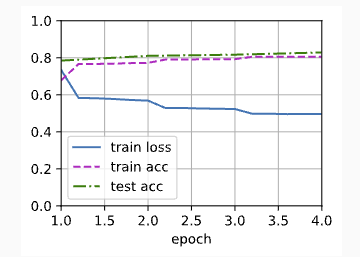
\includegraphics[height=4.1cm]{img/d2l_sentimento_rnn_treino.png}

            {\tiny Figura original do D2L, Seção 16.2.}
        \end{column}
    \end{columns}
    \begin{exampleblock}{Como ler o gráfico}
        \footnotesize
        A linha \textbf{verde} (\textit{test acc}) é a que importa: $\approx 83\%$ de acerto em críticas \textbf{nunca vistas}. Treino e teste próximos $\Rightarrow$ sem \textit{overfitting}.
    \end{exampleblock}

    \note{
        Por fim, o treino e os resultados.
        O otimizador é o Adam, com taxa de aprendizado 0,01. Ele adapta o tamanho do passo para cada parâmetro, e é muito usado em PLN por ser robusto. A perda é a entropia cruzada, que compara os dois logits com o rótulo certo, 0 ou 1. Os lotes têm 64 críticas.
        Este é o gráfico original do livro. Em azul, a perda de treino cai de cerca de 0,7 para perto de 0,49: o modelo erra cada vez menos. Em roxo tracejado, a acurácia de treino sobe até cerca de 0,80.
        E a linha verde, a acurácia no teste, é a mais importante: ela fica em torno de 0,8 e termina perto de 0,83. Isso quer dizer que o modelo acerta 83\% das críticas que nunca viu. Se a verde começasse a cair enquanto a roxa subisse, seria sinal de overfitting: o modelo teria decorado o treino. Como as duas estão próximas, o modelo está bem ajustado.
        Um detalhe curioso: o teste fica um pouco acima do treino. Isso acontece porque a acurácia de treino é a média ao longo da época, enquanto os pesos ainda estão mudando; a de teste é medida no fim da época, com o modelo já melhor.
        E, para fechar, as previsões do livro: ``this movie is so great'' sai positivo, e ``this movie is so bad'' sai negativo.
    }
\end{frame}
